\subsection{Earth-Sun system}

\subsubsection{Stability}

\begin{figure}[H]
    \centering
    \begin{subfigure}{0.5\textwidth}
        \centering
        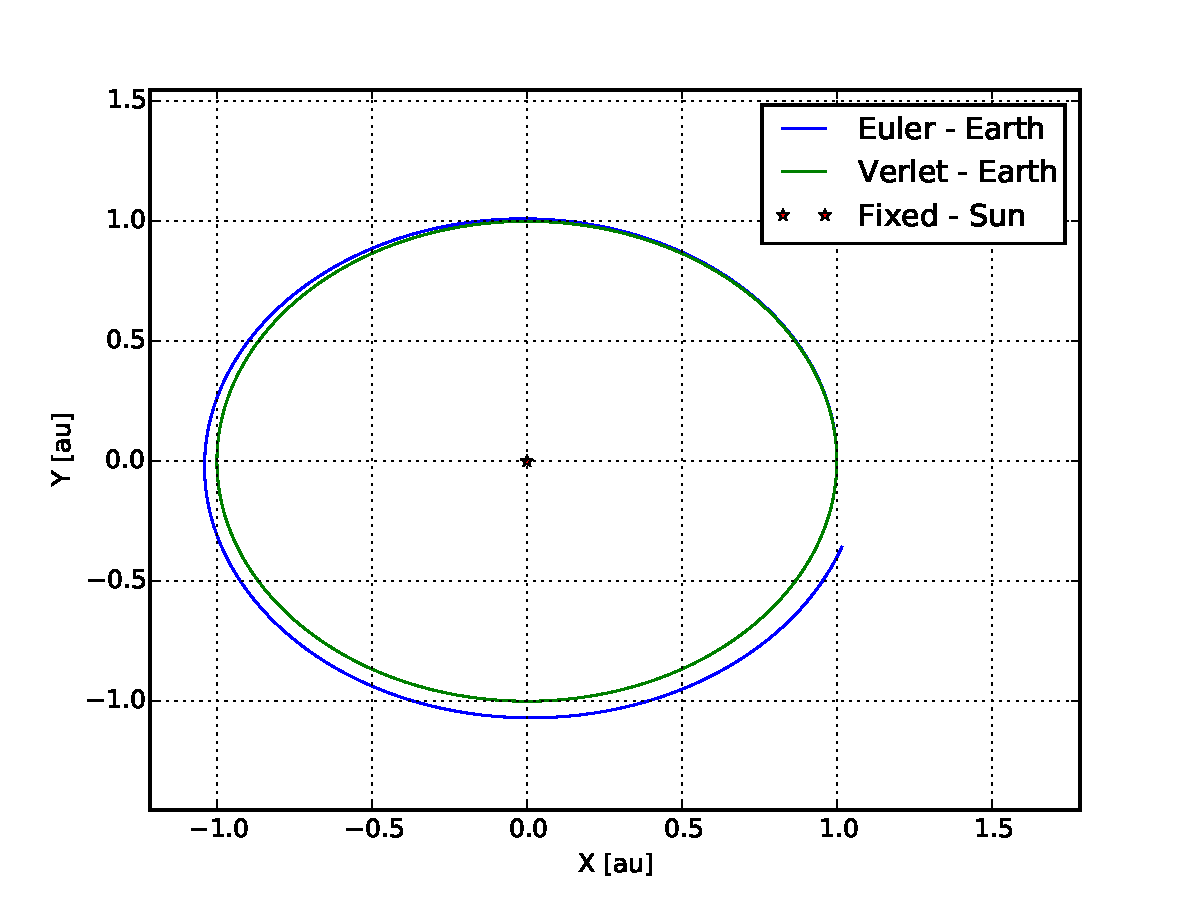
\includegraphics[width=\linewidth]{result/bilder/earth-sun.pdf}
    	\caption{}
    \end{subfigure}%
    ~ 
    \begin{subfigure}{0.5\textwidth}
        \centering
        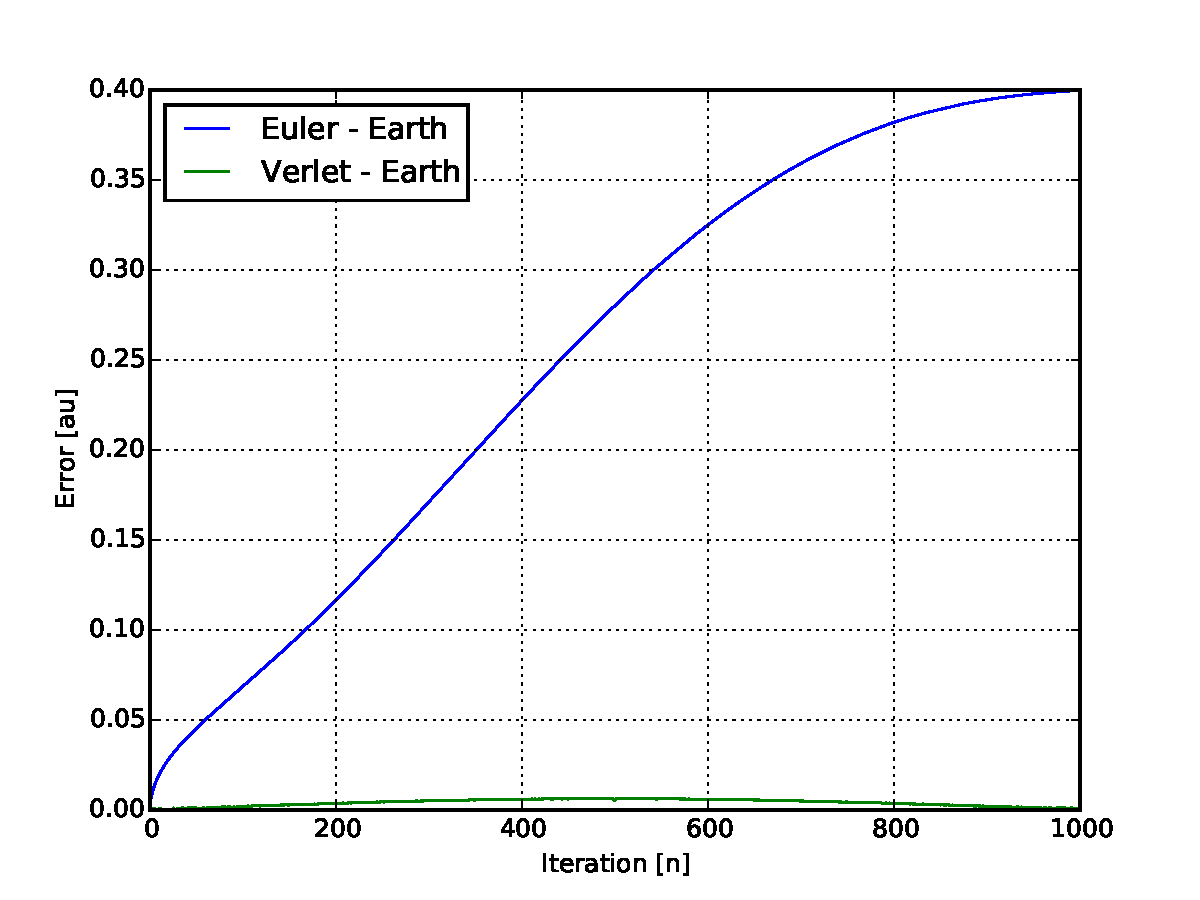
\includegraphics[width=\linewidth]{result/bilder/earth-sun-error.pdf}
        \caption{}
    \end{subfigure}
    \caption{a) show the orbit of earth around the sound. The intial velocity is set to $2\pi$ in y direction and the start position to 1 au in x direction. b) shows how the error behaves. The intial values should give a perfect circular motion. So the error is calculated by $r_i - r_{0}$. It is clear that Verlet-Velocity method is superior. This simulation was with 1000 points with the end time of 1 year. Both simulations was produced by \href{https://github.com/erikfsk/Project-3/blob/master/Project3/3a/plot_earth_sun.py}{\textcolor{blue}{plot\_earth\_sun.py}}}
    \label{fig:earth-sun}
\end{figure}


\subsubsection{Conserved quantities}

%\subsubsubsection{Kinetic energy}

%\subsubsubsection{Potential energy}

%\subsubsubsection{Angular momentum}

\subsubsection{Escape velocity}

%\subsubsubsection{$r = 1$ A.U. and dependent on $r^2$}

%\subsubsubsubsection{Trial and error answer}

%\subsubsubsubsection{Numerical answer}


%\subsubsubsection{Varying dependency of radius}



\subsection{Three body system}

\subsubsection{Fixed mass for jupitur}


\subsubsection{Varying mass for jupitur}




\subsection{Solar system}


\subsubsection{Three planets and all moving}


\subsubsection{Solar system all moving}





\subsection{The perihelion precession of Mercury}

\subsubsection{missing this part}